% !TEX root = single_chapter_sn1006.tex
\chapter{SN1006}
\label{chap:sn1006}


\section{Introduction}

\citet{1980ApJ...241.1039S} identified an unusual O-Star (now called Schweizer-Middleditch Star, henceforth \smstar) near the centre of SN1006. After successful identifications of neutron stars in both the Vela Remnant and the Crab Remnant this was thought to be the third identification of a stellar remnant in ancient supernovae. Subsequent UV spectroscopy follow-up of the \smstar by \citet{1983ApJ...269L...5W} , showed strong \ion{Fe}{2}  with a profile broadened by a few thousand \kms. In addition, \citet{1983ApJ...269L...5W} identified redshifted \ion{Si}{2}, \ion{Si}{3} and \ion{Si}{4} lines. Their conclusion was that these absorption lines stem from an expanding iron core surrounded by a Silicon shell (similar what theoretical models suggest for a \sneia). This places the \smstar behind the remnant and it is thought to be unrelated to SN1006. 

\sn{1006} is the closest of the young \snia remnants. It's distance has been determined to 2.2\,\kpc\ by using optical proper motion methods and radial velocity measurements from the remnant expansion \citep{2003ApJ...585..324W}. The remnant of \sn{1006}{} has been very well studied in many aspects. Absorption lines of the remnant plasma can be seen in background UV sources. This has enabled \citet{2005ApJ...624..189W} to sketch the inner structure of the ejecta. A few tenth of a solar mass of iron suggests that this event was a \snia. The lack of a neutron star, similar to those found in \snii remnants, also suggests a thermonuclear event. 

\sn{1006}{} provides the perfect site for a donor star search. High extinction values that introduce additional challenges to stellar analysis (as seen in the \sn{1572}{} remnant) are not present. The extinction, estimated for the background \smstar, is relatively low  at E(B-V) = 0.1 \citep{1993ApJ...416..247W,2003ApJ...585..324W}. These serendipitous conditions for the \sn{1006}{} remnant led us to launch a photometric and spectroscopic campaign to search for the donor star. The photometric observations were taken at Siding Spring Observatory with the 2.3m Telescope imager. The spectroscopic search area was determined by the center of the \snr{1006}{} and a radius (see Figure \ref{fig:overview_sn1006}). For the center we have opted to adapt a center determined by the mean of the \xray\ and radio center presented in \citet{2003ApJ...585..324W}. As a radius we have opted to use 120\arcsec, which translates into 1200\,\kms at the distance of \sn{1006}{}. We do believe that this generously chosen radius takes uncertainties of the center as well as the donor star scenarios into account. The spectroscopic observations were undertaken with the FLAMES multi-object spectrograph.

\begin{figure}[htbp] %  figure placement: here, top, bottom, or page
   \centering
   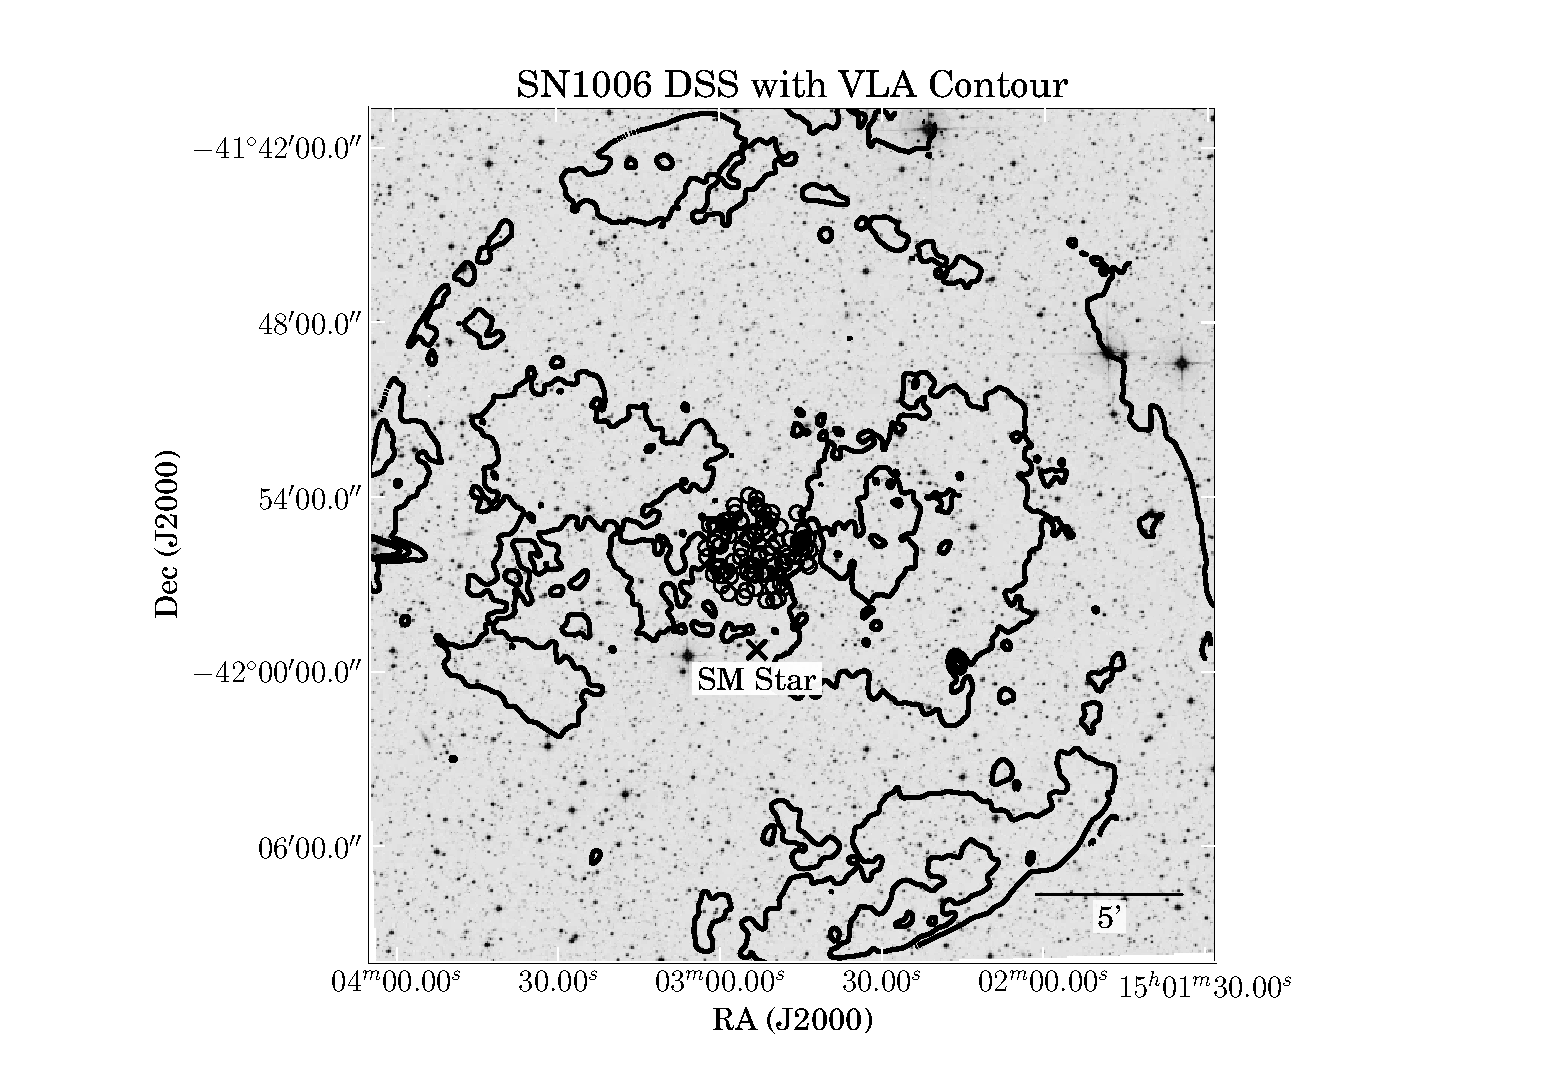
\includegraphics[width=0.8\textwidth]{chapter_sn1006/plots/sn1006_overlay_withsm.pdf} 
   \caption{example caption}
   \label{fig:overview_sn1006}
\end{figure}

We present photometry as well as high-resolution spectroscopy of the stars in SN1006 (for an overview see Figure \ref{fig:overview}. In Section \ref{sec:obs_and_red} we outline the observations as well as data reduction of the photometric and spectroscopic data. Section \ref{sec:analysis} is split into five subsections. We first describe the photometric analysis and radial velocity measurements. The complete analysis of the data has not been done and we mainly present our technique. We conclude this chapter in Section \ref{sec:conclusion} and discuss the possible implications of our initial find. In addition, we will describe future work including the final analysis of the data 


\section{Observations and Data Reduction}

For our spectroscopic survey we selected 79 stars in a 120 \arcsec radius (this corresponds to 780\,\kms at a distance of 2.2\,\kpc) around the centre of SN1006 ($\alpha = \rasc{15}{02}{22}{1};\delta = \decl{-42}{05}{49}$). We observed targets to a maximum magnitude of R=18, this translates to a limiting luminosity of $L=L_{\textrm{R}_\odot}$. The surviving donor scenarios described in \citet{2000ApJS..128..615M} and \citet{2008A&A...489..943P} should be easily visible at that photometric depth. 
The VLT instrument FLAMES provides high resolution (R=25,000) and a large field of view (25\arcmin) for a considerable number of stars per setup (130 targets). We chose the wavelength region from 5139\,\AA\ to 5356\,\AA\ which contains the gravity sensitive MgB Triplet as well as many Fe-Lines to accurately measure metallicity. Fibre buttons can be placed no less than 11\arcsec\ apart. Thus to observe all of the program stars in the crowded central field, we split the stars over three different setups. The first two setups were observed five times with 2775 s each. We deliberately chose bright stars for the last setup so that it only had to be observed three times with 2775 s each. As only the central 120\arcsec were crowded we placed spare fibres on three bright stars (R$\approx 10$; 2mass J15032744-4204463, J15031746-4204165, J15033195-4202356) located close to the edge of the 25\arcmin field for calibration purposes. Additional spare fibres were placed on sky positions. These were determined to be far from \twomass\ sources and were subsequently manually inspected using DSS images (citedss). 

We requested standard daytime calibration as well as simultaneous arc exposures with four fibres for each observation block. There are 13 observation blocks with an exposure time of 2775 s each. Table \ref{tab:observations} provides the Observing ID, modified julian date, mean seeing, mean airmass, setup name and heliocentric correction for all observations. Due to broken fibres not all stars where observed for the expected length of time. \candstar{31} was not observed at all in this sample (see Figure \ref{fig:zoomed_overview_sn1006} for the observation of the center of SN1006. This).

We applied a cosmic ray removal tool on the raw 2D frames \citep{2001PASP..113.1420V}. The data was then reduced with the ESO-CPL pipeline (version 5.2.0), using the GIRAFFE instrument recipes (version 2.8.9). The only change that was made to the default parameters was the usage of the Horne extraction algorithm instead of the "Optimal"-extraction algorithm. This yielded 366 individual spectra of the candidate stars and an additional 39 spectra of the Calibration stars. 
In addition, the Giraffe pipeline yields error frames which were used in the fitting process described in Section \ref{sec:sn1006_stelparam}. 
\begin{deluxetable}{cccccc}
\tablecaption{Observations}
\tablehead{\colhead{ObsID} & \colhead{MJD} & \colhead{FWHM} & \colhead{Airmass} & \colhead{SetupName} & \colhead{$\Delta v_{\rm helio}$}\\ 
\colhead{-} & \colhead{d} & \colhead{\arcsec} & \colhead{-} & \colhead{-} & \colhead{\kms}}


\startdata
360737 & 54965.1 & 1.2 & 1.2 & SN1006 1 & 1.5\\
360739 & 54965.1 & 1.2 & 1.1 & SN1006 1 & 1.5\\
360740 & 54965.1 & 1.0 & 1.1 & SN1006 1 & 1.4\\
360741 & 54985.0 & 0.7 & 1.4 & SN1006 1 & -7.4\\
360742 & 54964.2 & 1.5 & 1.1 & SN1006 1 & 1.7\\
360743 & 54985.0 & 0.8 & 1.2 & SN1006 2 & -7.5\\
360745 & 54985.0 & 0.9 & 1.1 & SN1006 2 & -7.6\\
360746 & 54985.1 & 1.0 & 1.1 & SN1006 2 & -7.7\\
360747 & 54985.1 & 1.0 & 1.1 & SN1006 2 & -7.7\\
360748 & 54985.2 & 0.9 & 1.1 & SN1006 2 & -7.8\\
360749 & 54963.1 & 1.2 & 1.2 & SN1006 3 & 2.4\\
360751 & 54963.1 & 1.1 & 1.1 & SN1006 3 & 2.3\\
360752 & 54963.2 & 1.1 & 1.1 & SN1006 3 & 2.3\\
\enddata
\label{tab:observations}
\end{deluxetable}


Our photometry was deduced from images taken with the image at the 2.3m Telescope at the Siding Spring Observatory. All data was taken on the night of the 11th of May. We exposed for 1860 s in U-Band, 1490 s in B-Band, 788s in V-Band and 1860 s in I-Band. For calibration purposes we took images of the PG1633 and PG1047 standard star regions in the same filters. The seeing ranged between 1 and 2 \arcsec. 
The data was reduced in the standard way using PyRAF \footnote{PyRAF is a product of the Space Telescope Science Institute, which is operated by AURA for NASA.}.
Finally an astrometric solution was fitted using astrometry from the \twomass\ point source catalogue \citep{2006AJ....131.1163S}. 


\section{Analysis}

A uniform analysis of this set of data is technically challenging due to the large variation in spectral quality (see Figure \ref{fig:sn1006_comparespec}). We have explored multiple channels and believe that, although challenging, it is possible. We measure the radial velocity using the standard technique of cross-correlation \citep{1979AJ.....84.1511T}. 
It is crucial in our set to measure rotation, as this is one of key features of potential donor stars. In addition, a giant star with high rotation can be incorrectly identified as a main-sequence star without rotation. We are currently trialling multiple techniques for measuring stellar rotation. For identifying the fundamental stellar parameters we use a standard grid based approach. In the next sections we will give a detailed description of the methods used, but do caution the reader that this is work in progress and subject to change for the final publication.

\subsection{Photometry}
We used SExtractor \citep{1996A&AS..117..393B} to measure the magnitudes of the objects in the frames. We used the Stetson magnitudes \footnote{This research used the facilities of the Canadian Astronomy Data Centre operated by the National Research Council of Canada with the support of the Canadian Space Agency}  of our standard fields PG1633 and PG1047 to calibrate our magnitudes to a standard Bessel Filter system. 

The measured magnitudes were supplemented with near infrared magnitudes from the \twomass\ point source catalogue.
To check the photometric measurements we plotted the obtained B-V colours against the V-K colours and compared this to theoretical colours from \citep{2010A&A...512A..54C} in Figure \ref{fig:colour_check}.  \candstar1006{60} presents a strong outlier in this case. Inspecting ours as well as \twomass imagery we believe there to be a second source which would explain this behaviour. 

To compute temperatures from photometric colours we used the polynomials given in  \citep{2010A&A...512A..54C} and assumed an \feh of 0 for all stars in the first instance. The temperature polynomial coefficients incorporating the metallicity are particularly small for the V-J colour. If V-K was not available (as 2MASS did only provide upper limits for some of our program stars) we tried to use V-J colours. The calculated temperatures were only used as a first reference and we are trying to use the spectral information in our final temperature measurement.

Table \ref{tab:sn1006_photometry} provides an overview of the photometry. We have also included $\theta$ a angular distance of the star to the adopted center.

% !TEX root = ../single_chapter_sn1006.tex
\ctable[
pos=p,
%width=\textwidth,
doinside=\scriptsize,
caption=SN1006 photometry,
label=tab:sn1006_photometry]
{lccccccccccc}{}{\FL
Name & RA & Dec & $\theta$ & U & $\sigma_\textrm{U}$ & B & $\sigma_\textrm{B}$ & V & $\sigma_\textrm{V}$ & I & $\sigma_\textrm{I}$\\ 
 & hh:mm:ss & dd:mm:ss & $\arcsec$ & mag & mag & mag & mag & mag & mag & mag & mag\ML
 SN1006 01 & 15:02:58.27 & -41:55:20.9 & 67.8 & 16.03 & 0.02 & 14.76 & 0.00 & 13.50 & 0.08 & 12.30 & 0.18\\
SN1006 02 & 15:02:59.95 & -41:56:25.2 & 86.1 & 18.84 & 0.08 & 16.96 & 0.01 & 15.37 & 0.01 & 13.95 & 0.05\\
SN1006 03 & 15:02:51.80 & -41:56:39.9 & 49.8 & 16.16 & 0.02 & 15.86 & 0.01 & 15.04 & 0.01 & 14.23 & 0.09\\
SN1006 04 & 15:02:53.35 & -41:54:18.0 & 93.6 & 16.67 & 0.02 & 16.33 & 0.00 & 15.47 & 0.00 & 14.62 & 0.00\\
SN1006 05 & 15:02:49.97 & -41:56:23.9 & 45.7 & 16.90 & 0.03 & 16.41 & 0.00 & 15.50 & 0.01 & 14.65 & 0.00\\
SN1006 06 & 15:02:45.68 & -41:54:35.2 & 110.5 & 16.21 & 0.01 & 16.17 & 0.01 & 15.50 & 0.00 & 14.78 & 0.01\\
SN1006 07 & 15:02:51.19 & -41:55:58.5 & 19.8 & 17.62 & 0.05 & 16.91 & 0.02 & 15.90 & 0.01 & 14.92 & 0.02\\
SN1006 08 & 15:02:47.00 & -41:55:28.3 & 69.3 & 16.57 & 0.03 & 16.53 & 0.01 & 15.86 & 0.01 & 15.16 & 0.00\\
SN1006 09 & 15:02:55.07 & -41:57:14.4 & 86.6 & 18.46 & 0.20 & 17.73 & 0.01 & 16.58 & 0.01 & 15.53 & 0.02\\
SN1006 10 & 15:03:01.87 & -41:54:59.2 & 113.4 & 17.18 & 0.04 & 17.06 & 0.00 & 16.30 & 0.00 & 15.51 & 0.00\\
SN1006 11 & 15:02:56.05 & -41:54:53.5 & 68.1 & 17.02 & 0.03 & 17.12 & 0.00 & 16.33 & 0.05 & 15.61 & 0.01\\
SN1006 12 & 15:02:58.83 & -41:56:35.5 & 80.0 & 17.60 & 0.03 & 17.22 & 0.00 & 16.39 & 0.02 & 15.50 & 0.02\\
SN1006 13 & 15:02:49.22 & -41:57:31.1 & 107.6 & 17.93 & 0.09 & 17.41 & 0.01 & 16.49 & 0.00 & 15.74 & 0.06\\
SN1006 14 & 15:02:59.24 & -41:54:51.6 & 93.1 & 17.93 & 0.04 & 17.44 & 0.00 & 16.56 & 0.00 & 15.75 & 0.01\\
SN1006 15 & 15:03:00.33 & -41:56:29.8 & 91.9 & 17.81 & 0.01 & 17.42 & 0.01 & 16.63 & 0.01 & 15.87 & 0.04\\
SN1006 16 & 15:02:58.09 & -41:54:47.9 & 86.4 & 19.60 & 0.47 & 18.37 & 0.01 & 17.26 & 0.00 & 16.11 & 0.03\\
SN1006 17 & 15:03:02.49 & -41:55:46.7 & 107.7 & 17.45 & 0.02 & 17.40 & 0.00 & 16.66 & 0.04 & 16.02 & 0.13\\
SN1006 18 & 15:02:50.99 & -41:56:39.4 & 52.2 & 18.00 & 0.03 & 17.61 & 0.00 & 16.77 & 0.03 & 15.87 & 0.04\\
SN1006 19 & 15:02:50.12 & -41:57:05.5 & 80.1 & 20.28 & 0.00 & 18.75 & 0.01 & 17.39 & 0.01 & 16.01 & 0.00\\
SN1006 20 & 15:02:48.03 & -41:56:19.4 & 60.6 & - & - & 19.59 & 0.03 & 18.04 & 0.01 & 15.97 & 0.17\\
SN1006 21 & 15:02:58.44 & -41:54:50.1 & 87.5 & 20.60 & 0.00 & 18.47 & 0.01 & 17.36 & 0.01 & 16.30 & 0.03\\
SN1006 22 & 15:02:59.95 & -41:55:41.9 & 79.8 & 17.26 & 0.04 & 17.25 & 0.00 & 16.71 & 0.06 & 16.18 & 0.04\\
SN1006 23 & 15:02:43.94 & -41:56:15.4 & 102.3 & 19.62 & 0.32 & 18.50 & 0.01 & 17.39 & 0.00 & 16.24 & 0.01\\
SN1006 24 & 15:02:56.14 & -41:54:49.2 & 72.3 & - & - & 18.28 & 0.00 & 17.59 & 0.13 & 16.49 & 0.11\\
SN1006 25 & 15:02:59.79 & -41:56:43.2 & 93.1 & 17.75 & 0.01 & 17.64 & 0.06 & 17.03 & 0.02 & 16.35 & 0.03\\
SN1006 26 & 15:02:54.92 & -41:55:27.7 & 33.1 & 18.10 & 0.10 & 17.95 & 0.01 & 17.23 & 0.02 & 16.43 & 0.00\\
SN1006 27 & 15:02:52.72 & -41:55:58.9 & 7.6 & 18.61 & 0.08 & 18.26 & 0.02 & 17.47 & 0.03 & 16.64 & 0.05\\
SN1006 28 & 15:02:54.86 & -41:56:36.4 & 50.2 & 18.52 & 0.13 & 18.24 & 0.00 & 17.43 & 0.02 & 16.70 & 0.02\\
SN1006 29 & 15:02:51.84 & -41:54:47.9 & 64.5 & - & - & 19.23 & 0.00 & 18.00 & 0.02 & 16.72 & 0.04\\
SN1006 30 & 15:02:44.71 & -41:55:15.4 & 97.7 & 18.05 & 0.03 & 18.24 & 0.03 & 17.54 & 0.02 & 16.75 & 0.01\\
SN1006 32 & 15:02:53.61 & -41:55:13.7 & 38.7 & 18.72 & 0.18 & 18.42 & 0.02 & 17.64 & 0.03 & 16.78 & 0.03\\
SN1006 33 & 15:02:43.38 & -41:55:51.5 & 105.7 & 19.07 & 0.23 & 18.56 & 0.04 & 17.66 & 0.04 & 16.69 & 0.05\\
SN1006 34 & 15:02:56.13 & -41:56:05.1 & 39.1 & 18.64 & 0.11 & 18.52 & 0.02 & 17.76 & 0.01 & 16.94 & 0.01\\
SN1006 35 & 15:02:44.66 & -41:55:10.0 & 100.4 & 19.06 & 0.17 & 18.74 & 0.00 & 17.84 & 0.02 & 16.88 & 0.05\\
SN1006 36 & 15:02:58.70 & -41:55:02.9 & 81.4 & 19.46 & 0.40 & 18.65 & 0.01 & 17.79 & 0.01 & 16.86 & 0.02\\
SN1006 37 & 15:02:58.96 & -41:55:02.5 & 83.9 & - & - & - & - & - & - & - & -\\
SN1006 38 & 15:02:50.29 & -41:55:45.6 & 29.2 & 18.58 & 0.08 & 18.48 & 0.03 & 17.80 & 0.03 & 17.00 & 0.01\\
SN1006 39 & 15:02:43.76 & -41:55:25.6 & 104.7 & 18.86 & 0.06 & 18.44 & 0.02 & 17.69 & 0.01 & 16.97 & 0.01\\
SN1006 40 & 15:02:52.23 & -41:56:37.9 & 47.0 & - & - & - & - & - & - & 16.28 & 0.06\\
SN1006 41 & 15:02:52.06 & -41:55:05.2 & 47.1 & 17.97 & 0.01 & 18.02 & 0.00 & 17.61 & 0.01 & 17.11 & 0.02\\
SN1006 42 & 15:02:57.08 & -41:54:34.3 & 90.4 & 19.22 & 0.27 & 18.78 & 0.03 & 17.99 & 0.01 & 17.16 & 0.03\\
SN1006 43 & 15:02:48.27 & -41:56:15.9 & 56.7 & - & - & 20.14 & 0.04 & 18.76 & 0.08 & 17.25 & 0.06\\
SN1006 44 & 15:02:51.96 & -41:54:31.4 & 80.7 & - & - & 19.79 & 0.01 & 18.54 & 0.02 & 17.06 & 0.01\\
SN1006 45 & 15:02:47.43 & -41:56:05.3 & 62.0 & 18.45 & 0.11 & 18.43 & 0.02 & 17.71 & 0.03 & 17.00 & 0.05\\
SN1006 46 & 15:02:49.93 & -41:57:35.3 & 108.8 & 20.09 & 0.17 & 19.04 & 0.03 & 18.05 & 0.04 & 17.19 & 0.20\\
SN1006 47 & 15:02:52.86 & -41:54:25.7 & 85.7 & 18.89 & 0.24 & 18.63 & 0.01 & 17.96 & 0.03 & 17.14 & 0.03\\
SN1006 48 & 15:02:54.52 & -41:55:29.9 & 28.5 & - & - & 19.29 & 0.03 & 18.38 & 0.01 & 17.38 & 0.06\\
SN1006 49 & 15:02:52.83 & -41:56:06.1 & 14.7 & 18.90 & 0.33 & 18.84 & 0.00 & 18.17 & 0.01 & 17.37 & 0.05\\
SN1006 50 & 15:02:53.93 & -41:56:22.6 & 33.4 & 19.68 & 0.11 & 18.99 & 0.03 & 18.07 & 0.03 & 17.19 & 0.02\\
SN1006 51 & 15:02:54.58 & -41:53:58.4 & 114.7 & 19.47 & 0.00 & 18.90 & 0.26 & 17.99 & 0.19 & 16.93 & 0.17\\
SN1006 52 & 15:03:00.97 & -41:54:58.6 & 104.9 & 19.41 & 0.17 & 18.89 & 0.00 & 18.08 & 0.03 & 17.24 & 0.02\\
SN1006 53 & 15:02:57.45 & -41:56:14.7 & 56.4 & 19.32 & 0.43 & 18.90 & 0.03 & 18.13 & 0.01 & 17.24 & 0.05\\
SN1006 54 & 15:02:48.09 & -41:57:07.7 & 92.9 & 20.33 & 0.58 & 19.40 & 0.02 & 18.45 & 0.01 & 17.48 & 0.03\\
SN1006 55 & 15:02:44.67 & -41:55:35.9 & 92.6 & - & - & 19.90 & 0.01 & 18.68 & 0.03 & 17.36 & 0.04\\
SN1006 56 & 15:02:50.38 & -41:54:34.5 & 81.7 & - & - & 20.15 & 0.16 & 18.83 & 0.06 & 17.46 & 0.08\\
SN1006 57 & 15:02:54.15 & -41:56:40.9 & 51.5 & 19.59 & 0.57 & 18.91 & 0.02 & 18.26 & 0.04 & 17.63 & 0.07\\
SN1006 58 & 15:02:49.42 & -41:55:33.5 & 42.3 & 18.90 & 0.09 & 18.92 & 0.02 & 18.21 & 0.02 & 17.41 & 0.02\\
SN1006 59 & 15:02:51.38 & -41:57:34.9 & 104.7 & 19.59 & 0.37 & 19.21 & 0.01 & 18.54 & 0.02 & 17.78 & 0.02\\
SN1006 60 & 15:02:59.64 & -41:57:03.8 & 104.8 & 20.05 & 0.18 & 19.22 & 0.01 & 18.48 & 0.13 & 18.62 & 0.43\LL}

\ctable[
%width=\textwidth,
doinside=\scriptsize,
caption=SN1006 photometry,
continued,
label=tab:sn1006_photometry]
{lccccccccccc}{}{\FL
Name & RA & Dec & $\theta$ & U & $\sigma_\textrm{U}$ & B & $\sigma_\textrm{B}$ & V & $\sigma_\textrm{V}$ & I & $\sigma_\textrm{I}$\\ 
 & hh:mm:ss & dd:mm:ss & $\arcsec$ & mag & mag & mag & mag & mag & mag & mag & mag\ML
SN1006 61 & 15:02:53.45 & -41:57:09.2 & 78.0 & - & - & 20.49 & 0.05 & 19.24 & 0.02 & 17.82 & 0.07\\
SN1006 62 & 15:02:44.94 & -41:55:48.3 & 88.3 & - & - & 19.38 & 0.02 & 18.53 & 0.01 & 17.54 & 0.01\\
SN1006 63 & 15:02:50.89 & -41:55:17.4 & 40.5 & 20.19 & 0.15 & 19.41 & 0.00 & 18.55 & 0.02 & 17.62 & 0.05\\
SN1006 64 & 15:02:55.53 & -41:57:28.3 & 101.4 & 19.45 & 0.28 & 18.87 & 0.02 & 18.51 & 0.03 & 17.87 & 0.08\\
SN1006 65 & 15:02:44.57 & -41:55:28.2 & 95.3 & 18.79 & 0.04 & 18.93 & 0.03 & 18.38 & 0.04 & 17.63 & 0.05\\
SN1006 66 & 15:02:57.28 & -41:54:19.6 & 104.3 & - & - & 20.02 & 0.03 & 19.09 & 0.02 & 18.00 & 0.03\\
SN1006 67 & 15:02:48.88 & -41:55:03.4 & 65.4 & 19.69 & 0.38 & 19.11 & 0.03 & 18.37 & 0.01 & 17.57 & 0.01\\
SN1006 68 & 15:02:43.51 & -41:56:23.9 & 109.2 & 20.65 & 0.00 & 19.60 & 0.04 & 18.75 & 0.04 & 17.94 & 0.01\\
SN1006 69 & 15:03:01.11 & -41:56:40.2 & 104.3 & 20.07 & 0.00 & 19.59 & 0.03 & 18.59 & 0.17 & 17.91 & 0.09\\
SN1006 70 & 15:02:58.01 & -41:56:45.0 & 78.6 & 20.38 & 0.57 & 19.49 & 0.01 & 18.73 & 0.03 & 18.00 & 0.06\\
SN1006 71 & 15:03:00.93 & -41:55:35.3 & 91.6 & - & - & 19.95 & 0.02 & 18.84 & 0.02 & 17.92 & 0.25\\
SN1006 72 & 15:02:58.39 & -41:57:20.6 & 108.5 & 19.34 & 0.00 & 19.90 & 0.11 & 18.85 & 0.11 & 18.01 & 0.14\\
SN1006 73 & 15:02:50.64 & -41:54:49.5 & 66.7 & - & - & 20.00 & 0.04 & 19.04 & 0.06 & 17.92 & 0.12\\
SN1006 74 & 15:03:02.32 & -41:56:05.2 & 106.6 & - & - & 19.88 & 0.08 & 18.76 & 0.16 & 18.21 & 0.02\\
SN1006 75 & 15:02:53.19 & -41:54:05.5 & 106.0 & 19.23 & 0.11 & 19.07 & 0.03 & 18.34 & 0.03 & 17.50 & 0.03\\
SN1006 76 & 15:02:44.17 & -41:55:45.8 & 97.0 & 19.56 & 0.09 & 19.40 & 0.02 & 18.70 & 0.03 & 17.91 & 0.08\\
SN1006 77 & 15:02:55.98 & -41:55:47.4 & 35.2 & 19.58 & 0.20 & 19.22 & 0.02 & 18.56 & 0.05 & 17.69 & 0.02\\
SN1006 78 & 15:02:48.76 & -41:56:59.9 & 82.3 & - & - & 20.87 & 0.10 & 19.53 & 0.01 & 18.06 & 0.05\\
SN1006 79 & 15:02:53.45 & -41:56:41.7 & 50.7 & - & - & 21.53 & 0.06 & 19.90 & 0.02 & 18.04 & 0.05\\
\LL}


\subsection{Proper motion}
Do we have proper motions? We claimed to have some to an accuracy of 10 mas/yr in our ESO proposal. I will leave this section out I think. 

\subsection{Radial Velocity}

To obtain radial velocities we employ a two step process. We first used a solar spectrum from \citep{1984sfat.book.....K} with the standard cross-correlation technique described in \citep{1979AJ.....84.1511T} and implemented in the IRAF-task \textit{fxcor}. The cross-correlation was performed on every single spectra. The results were then heliocentrically corrected, then averaged for each star with a sigma clipping algorithm. We note that especially for faint objects we observe a second cross-correlation peak at 0\,\kms and believe that this is reflected light from the moon. We believe that this has a negligible effect on our cross-correlation and the measurement of stellar parameters. This is the current progress for radial velocity measurements. As a future step we will remeasure the radial velocity with a matching template spectrum, although we do believe that this won't change the current results significantly.

In Figure \ref{fig:sn1006_vrad_comp} we have compared our radial velocity measurements with the Besan\c{c}on kinematic model of the Milky way \citep{2003A&A...409..523R}. The selection criteria for creating the  Besan\c{c}on kinematic model was all stars a circle around \sn{1006}{} with an area 1 square degree and a magnitude cut of $\textrm{V}>10$. We compared the resulting 16400 stars to our 78 stars in the sample. 


\begin{figure}[htbp] %  figure placement: here, top, bottom, or page
   \centering
   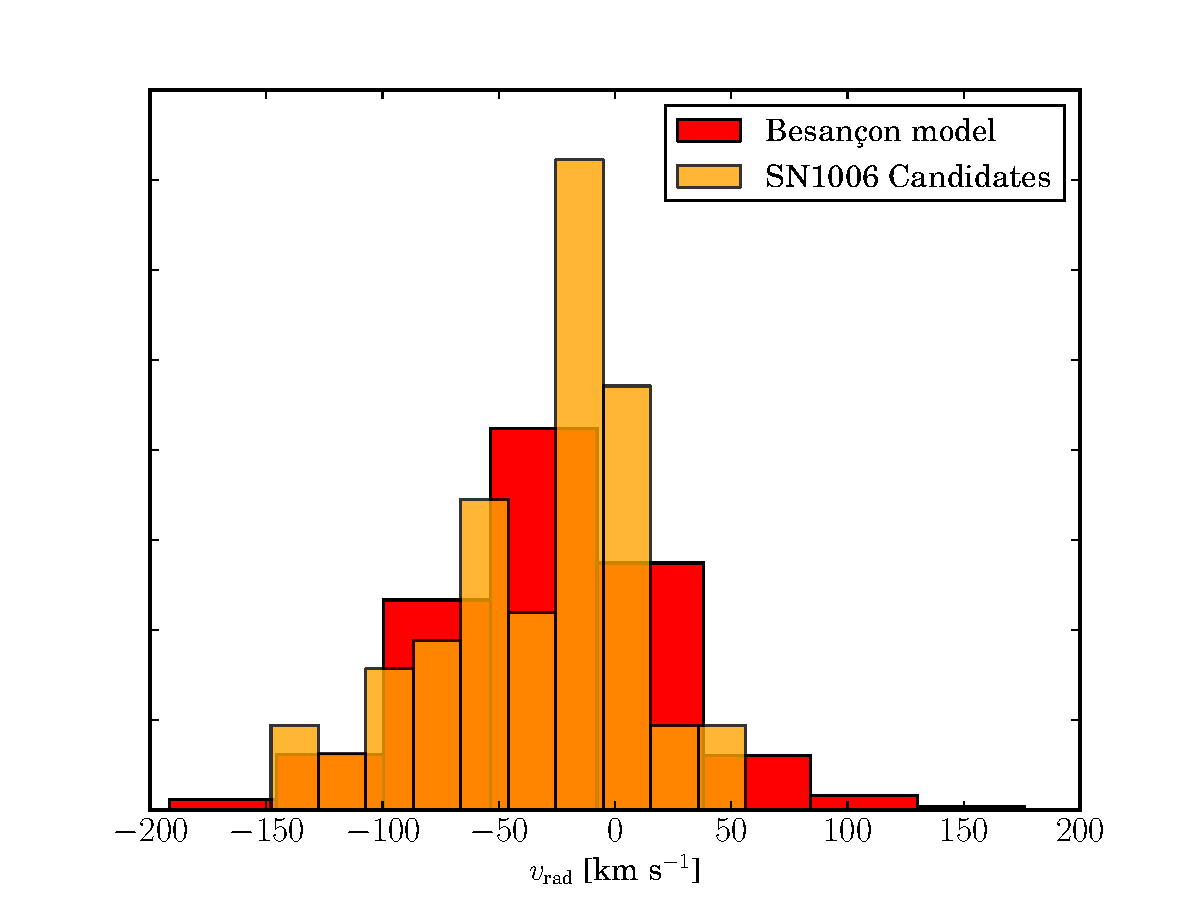
\includegraphics[width=0.7\textwidth]{chapter_sn1006/plots/sn1006_vrad_besancon.pdf} 
   \caption{example caption}
   \label{fig:sn1006_vrad_comp}
\end{figure}


\subsection{Rotational Velocity}
\label{sec:sn1006_rotvel}
There is a large velocity spread in the direction of \sn{1006}{} (see Figure \ref{fig:sn1006_vrad_comp}). This makes it hard to isolate a donor star just on kinematic features. A distinguishing feature for a donor star might be rotation (discussed in  Chapter \ref{chap:sn1572_starg}). The rotational velocities in Chapters \ref{chap:sn1572_starg} and \ref{chap:sn1572_hires} were all measured manually. We selected weak iron lines and stacked them to obtain a line profile, which was compared to synthetically rotationally broadened lines. This was a feasible way for six spectra, it is however not feasible for more than 300 spectra. 

Initially we had tried to fit the rotational velocity as an additional parameter in the determination of stellar parameters. For the low signal to noise spectra the optimization algorithm suggested very high rotations. A simple manual inspection revealed that this was not the case. In fourier space (priv. communication Ken Freeman) it becomes much easier to determine repetitive  structures like line profiles. Initially we tried a simple fourier transform of the spectra without using a window function. This caused a very noisy fourier spectrum, which was hard to analyse. \cite{citeulike:8297810}, on the other hand describes a very robust method of obtaining periodic information of spectra.  He suggests dividing the spectra into overlapping subsegments. These are then multiplied with a window function (in our case ``Hann''-window) and transformed into the fourier domain. All fourier segments are then averaged, which provides a very clean fourier spectrum. Figure \ref{fig:sn1006_psd} shows the periodogram of synthetic spectra with different rotation and different S/N-ratios. For synthetic data this methods worked even for a S/N of roughly 5. Measuring rotation in our real data remained too difficult in the low S/N regime. 

%picture: This reduces removes the low frequencies and reduces frequency resolution. In our case, however, we are interested in high frequency caused by the line profiles. 
We however discovered a different way of measuring line profiles (and inferring rotation). For a description of this method we review part of the spectrum synthesis. The intrinsic spectrum ($f_\textrm{spectrum}$)is created at the photosphere of the star (but already broadened by many factors like thermal broadening). A rotation of that star convolves the spectrum with a rotational broadening kernel ($g_\textrm{rotation}$). The light travels to earth and then is convolved again with the instrument profile ($h_\textrm{instrument}$) before being recorded on the detector.  Let's assume we can create a synthetic spectra matching the intrinsic stellar one which has not been convolved by either rotation or the instrument ($f_\textrm{synthetic}$). A convolution can be described in Fourier space in the following way,
\begin{align*}
	f_\textrm{observed} =& f_\textrm{spectrum} \otimes \underbrace{g_\textrm{rotation} \otimes h_\textrm{instrument}}_{f_\textrm{profile}}\\
     F(f_\textrm{spectrum} \otimes g_\textrm{rotation} \otimes h_\textrm{instrument}) =& F(f_\textrm{spectrum}) \times F(g_\textrm{rotation}) \times F(h_\textrm{instrument})\\
     \Rightarrow \frac{F(f_\textrm{observed})}{F(f_\textrm{synthetic})} \approx& F(f_\textrm{profile}),
\end{align*}
where $F$ denotes the fourier transform. This yields the line profile which we can roughly separate into the instrument profile (using prior knowledge about the resolution of the instrument) and a rotational kernel . This technique is by no means a new idea. It has been described by a selection of authors \citep[e.g.][]{1977ApJ...211..198G}. This is the basic method that \textit{fxcor} relies on. \textit{fxcor} however only measures the peak of the profile to estimate the radial velocity. Our collaborator John Laird has used this technique to successfully extract the rotation for some of the stars (see Table \ref{tab:sn1006_stelparam}). We are planning to combine the previously described Welch's method and this fourier cross-correlation to reliably measure rotation in low S/N data. This is currently still research in progress.

\subsection{Stellar Parameters}
\label{sec:sn1006_stelparam}

To get detailed stellar parameters we employ a technique using a grid in \teff, \logg\ and \feh. 
\moog \citep{1973ApJ...184..839S} was used to synthesize the spectral grid using the model stellar atmospheres by \citet{2003IAUS..210P.A20C}. Line wings were taken into account up to 8\,\AA away from line centre, which seemed to be a reasonable compromise between grid creation time and accuracy. For the atomic lines we merged values from the VALD-2 database \citep{2000BaltA...9..590K} with adjusted values (to reproduce the Arcuturs and the Sun) from \cite{2008A&A...486..951G}. We used the measured
molecular lines described in  \citet{1995KurCD..23.....K}. 
The grid extends from 3500\,K to 7500\,K in \teff with a stepsize of 250\,K, in \logg\ it ranges from  0 to 5 with a stepsize of 0.5 and in \feh\ it ranges from -2.5 to 0.5 with a stepsize of 0.5 (with an extra set of points at 0.2). 

We used the appropriate sections from the Solar spectrum \citep{1984sfat.book.....K} and the Arcturus spectrum  \cite{2000vnia.book.....H} to calibrate our spectral grid. We determined stellar parameters by first finding the best fitting grid point and then using the minimizer MINUIT to find a minimum by interpolating between the gridpoints \citep[using][]{Barber96thequickhull}. For a more detailed explanation of the n-dimensional interpolation see chapter \ref{chap:ndinterp}. For the Sun we obtain stellar parameters of \teff=5825\,K, \logg=4.4 and \feh=-0.12 and for Arcturus we obtain stellar parameters of \teff=4336\,K, \logg=1.9, \feh=-0.67. We acknowledge the error in measurement, but believe our spectral grid to be accurate enough for distinguishing a potential donor candidate against an unrelated star. 


To measure our observed spectra we need to first fit the continuum. We decided for a Legendre polynomial with a maximum order of 3 and a sigma clipping algorithm. The order that gave the lowest RMS of the fit was used. After determining initial parameters we would divide by synthetic spectrum with these parameters and fit the continuum again as some parameters (like \feh) are very continuum sensitive.  

To calibrate this analysis pipeline we have measured stellar parameters for synthetically created spectra using the real sun and arcturus spectra as an input. We multiplied these spectra with an artificial continuum and introduced artificial noise to recreate a S/N-ratio of 5 (similar to the measure low S/N spectra) and added rotation in some cases. Both Solar and Arcturus spectrum were introduced into the analysis pipeline with artificially added noise and rotation. As rotation can not yet be reliably identified by our techniques (see Section \ref{sec:sn1006_rotvel}) we sometimes obtained measurements that suggested a rotationally convolved Arcturus to be a main-sequence. As higher surface gravity broadens the wings of some spectral lines, our algorithm confused the rotational broadened lines of the artifically rotating Arcturus spectrum with gravity broadening. 

In summary, we have not yet been able to reliably extract stellar parameters from the observerd spectra. Initial experiments with the low S/N spectra of individual stars often yielded the same parameters for the same star. This is a promising result and suggests, that if we can reliably determine the line profile we will be able to extract stellar parameters for the candidates.


\section{Conclusions}

The initial measurements of kinematics, photometric temperatures and initial rotational velocities suggest no unusual stars in the current set. None of the stars show any particularly peculiar radial velocity. We note however that the spread in radial velocity in this direction is large and that a potential donor star might not be visible as a kinematic outlier. The current measurements of rotation also do not show any strong outliers.
Once we obtain measurements about evolutionary and more precise measurements about the temperatures we will be able to infer distances. The relatively low reddening of the field will make this a straightforward exercise. Distances often offer suggestive evidence for involvement (e.g. \starg in SN1572). If the further analysis does not, as currently hinted, reveal an unambiguously identifiable donor star for \sn{1006}{} we will have have to analyze the caveats of such a find. In our opinion the determination of the center is one of the largest caveats. Measurements like \citet{2005ApJ...624..189W} cast doubt on a precise determination of the center. Their research suggests that the center of the iron core is offset from the geometric center determined by the shocked \ism. This does, however, not mean that the center of mass (where a donor star would reside) is necessarily offcenter. In fact, \cite{2010ApJ...708.1703M} suggest that the innermost ejecta is offset from the center of mass, which suggests that the center of the iron core will be different than the center of mass. In summary, this caveat is probably not easily resolved and we will have to hope that our generous choice in radius around the geometric center incorporates any such errors. Other groups are also currently surveying SN1006 with in a larger but photometrically shallower field (priv. communication Pilar Ruiz-Lapuente). Their search also has not revealed any unusual star. Finally, the donor star that we are trying to find might already be to faint for our observations. Although scenarios with very faint stellar remnants exist, most current scenarios do not suggest this (see discussion in section \ref{sec:donor star}.) The other very real possibility is that \sneia\ in general or at least \sn{1006}{} did not have a donor star. A \dd-scenario would definitley explain the observational lack of the thought after companion. 
Finally, the last remnant to be subjected to such an intensive search will be Kepler. Kepler seems to be different from either SN1572 and SN1006 due to detection of interaction with \csm. Observational facts of the Kepler remnant (SN1604) as well as the description of the donor star search will be discussed in \ref{chap:conclusion}

